\section{Fluxograma do Software}

\begin{figure}[!htb]
    \centering
    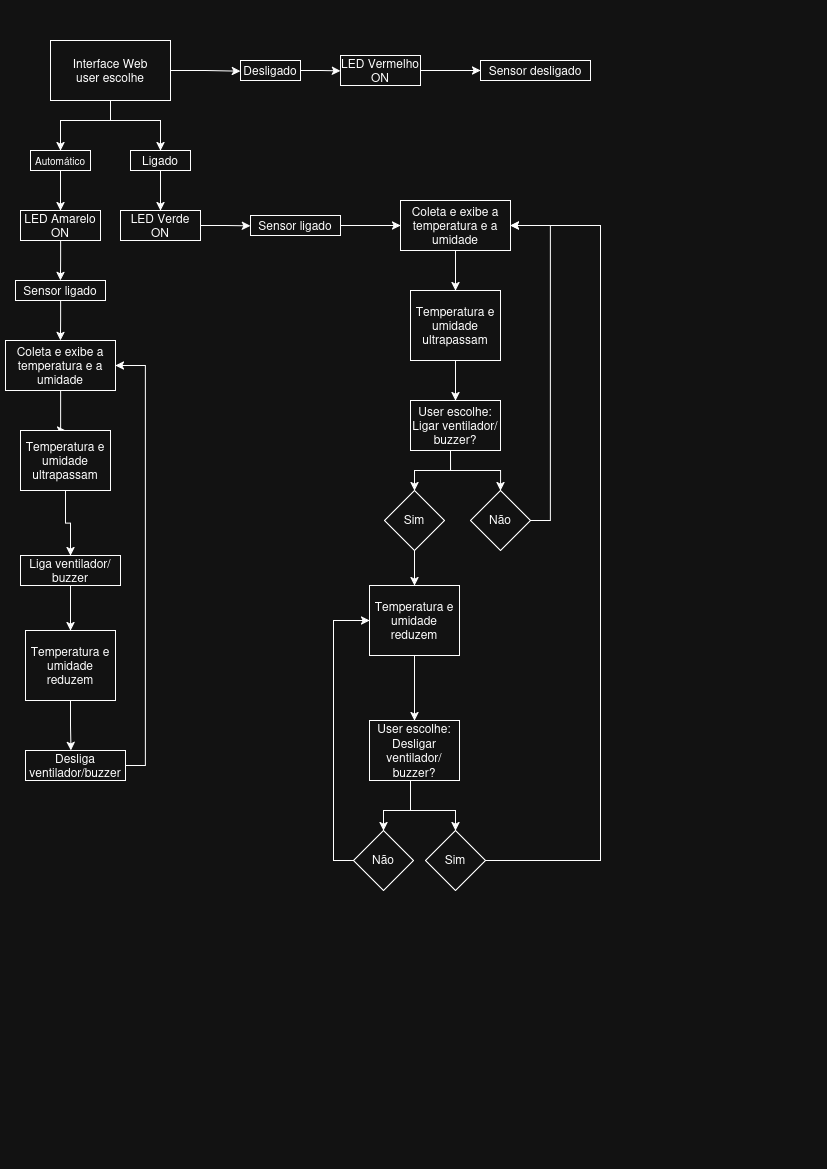
\includegraphics[width=0.7\textwidth]{imag/Fluxograma.png}
    \caption{Fluxograma de funcionamento do software do sistema.}
    \label{fig:fluxograma_software}
\end{figure}

O fluxograma da Figura \ref{fig:fluxograma_software} representa a lógica de execução do software embarcado. O sistema parte da escolha do usuário na interface web entre os que seguem abaixo:

\begin{itemize}
    \item \textbf{Desligado:} o LED vermelho é aceso e o sensor é desligado, interrompendo a coleta de dados;
    \item \textbf{Automático:} o LED amarelo é aceso e o sensor coleta e exibe os dados continuamente. Se as leituras ultrapassarem os limites, o sistema aciona sozinho o ventilador e o buzzer, desligando-os quando os valores voltam ao normal;
    \item \textbf{Ligado (Manual):} o LED verde é aceso e o sensor coleta e exibe os dados em tempo real. Se os limites forem ultrapassados, o sistema pergunta ao usuário, pela interface, se deseja acionar o ventilador e o buzzer, e repete a consulta para desligá-los.
\end{itemize}
